%%%%%%%%%%%%%%%%%%%%%%%%%%%%%%%%%%%%%%%%%
% Szablon pracy dyplomowej
% Wydział Informatyki 
% Zachodniopomorski Uniwersytet Technologiczny w Szczecinie
% autor Joanna Kołodziejczyk (jkolodziejczyk@zut.edu.pl)
% Bardzo wczesnym pierwowzorem szablonu był
% The Legrand Orange Book
% Version 5.0 (29/05/2025)2023)
%
% Modifications to LOB assigned by %JK
%%%%%%%%%%%%%%%%%%%%%%%%%%%%%%%%%%%%%%%%%s

\chapter{Swagger}
\label{chapter:dodatek_A}

\textit{Poniżej przedstawiono interfejs Swagger prezentujący dostępne endpointy API oraz struktury danych.}

\begin{figure}[!htb]
	\centering
	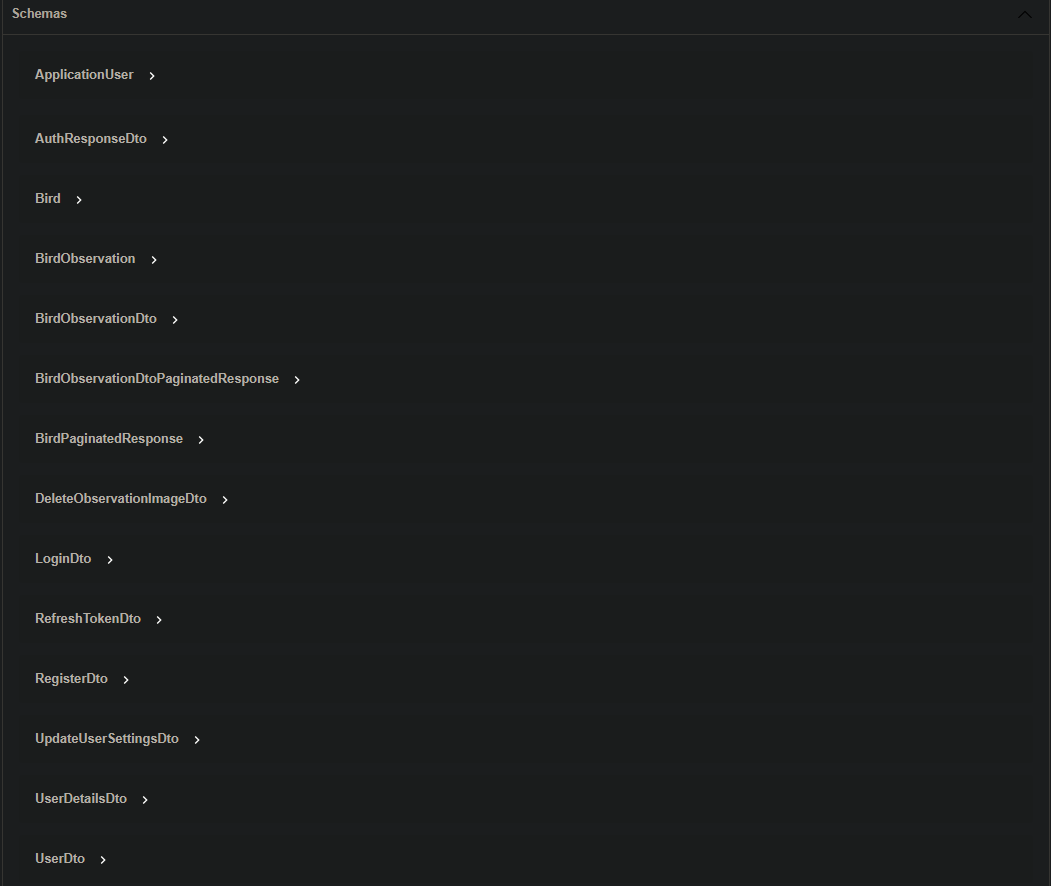
\includegraphics[width=1.0\textwidth]{/dodatekA/Swagger2.png}
	\caption{Interfejs Swagger struktury}
	\label{fig:swagger2}
\end{figure}

\begin{figure}[!htb]
	\centering
	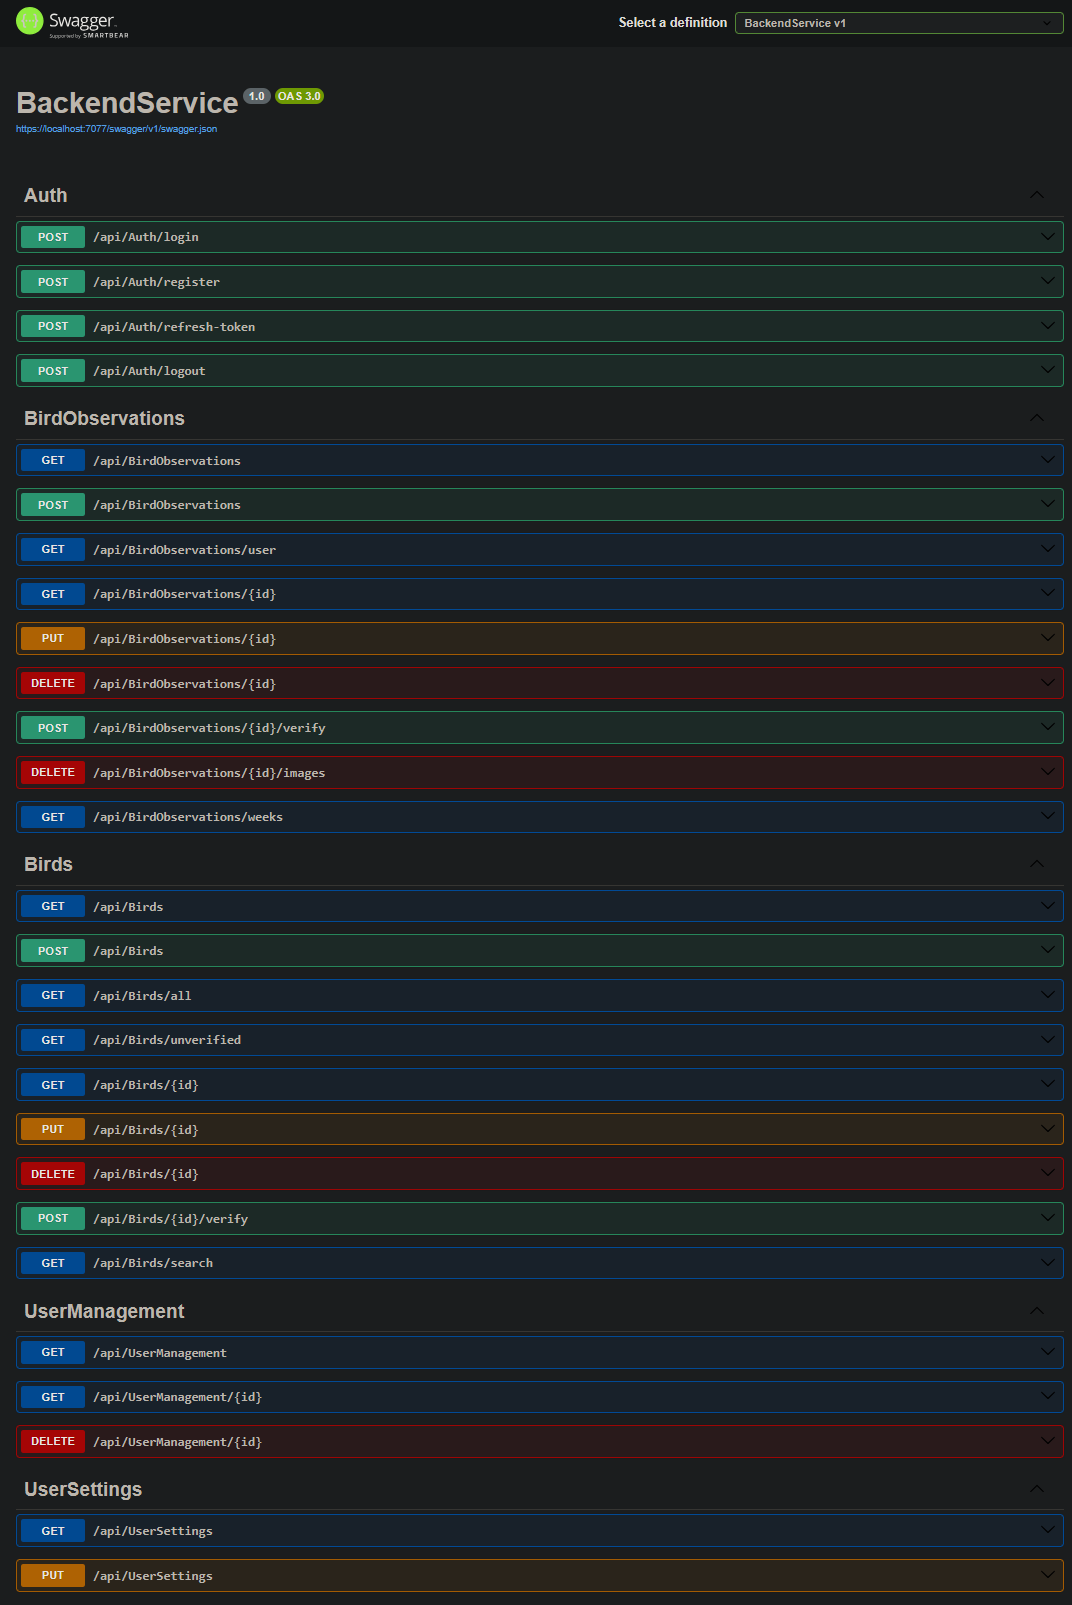
\includegraphics[width=1.0\textwidth]{/dodatekA/Swagger1.png}
	\caption{Interfejs Swagger endpointy}
	\label{fig:swagger1}
\end{figure}